\section{interfaces}
    \subsection{Introduction}
        Pour représenter notre jeu, nous avons donc créer 2 interfaces: une interface textuelle et une interface graphique. Afin de faciliter la transition entre ces deux interfaces et le programme du jeu, qui est donc le même peut importe l'interface, nous avons décidé de faire en sorte qu'elles aient toutes les deux la même structure. Elles sont ainsi simplement différentes dans la façon dont elles récupèrent/affichent les informations. C'est au début de la partie que l'une ou l'autre seront choisie par l'utilisateur via la console.
    \subsection{Interface Textuelle}
        Lorsque c'est l'interface textuelle qui est choisie, l'entièreté de la partie se déroulera alors dans la console, que ce soit les choix des joueurs ou les informations sur le déroulé du jeu. Au cours de la partie, les différents choix à effectuer par le/les joueurs humain(s) si il y'en a seront à taper directement dans la console (pour les ia seuls les résultats de leurs choix s'afficheront).
        Dans le cas de l'interface textuelle, une fonction 'input securise' assure la bonne comprehension des reponses des utilisateurs. Celle-ci ne laissent passer que des réponses pré-definies (ex: un nom de pokemon, un nom d'attaque) et permet ainsi d'éliminer les erreurs dûes aux réponses non-conformes des utilisateur (nom mal orthographié ou inexistant).
        \bigskip
            \subsubsection{déroulé d'un tour}
                Dans un premier temps, il faudra taper dans la console la nature des deux joueurs ainsi que leurs nom et leur pokemon de départ, en répondant aux questions correspondantes dans la console comme explicité ci-contre:(cf image 1 au point 6.2.2)
                
                \bigskip
        
                Pour chaque tour (après un récapitulatif des choix respectifs des deux joueurs si il s'agit du premier tour), les deux joueurs sont appelé à choisir ce qu'ils vont faire, en choisissant entre attaquer ou changer de pokemon, avec la possibilité d'avoir accès aux informations de la partie avant de choisir. Les différents choix d'attaque ou de pokemon posssible seront rappelés au joueur avant qu'il ne choisisse. Voici des exemples :(cf image 2 au point 6.2.2)
    
                \bigskip
    
                A la fin du tour, un résumé des différents actions ayant eu lieu durant ce tour sera affiché dans la console, accompagné d'un bilan global de l'état du jeu à ce tour, avec les informations sur les pokemons des deux joueurs commme présenté ci-contre:(cf image 3  au point 6.2.2)

                \bigskip

                Enfin, lorsque qu'un joueur n'a plus de pokemon en état de combattre, un message vient annoncer le vainqueur et la fin de la partie.(cf image 4  au point 6.2.2)

            \bigskip
            
            \subsubsection{affichages en textuel:}
                Touts les affichages de l'interface textuelle sont gérés par des print appliqués par les différentes fonction de la classe InterfaceTexte ou par le fichier jeu (voir architecture du programme) pour ce qui concerne les informations destinées aux utilisateur et par la fonction 'input securise' pour ce qui concerne les informations données par l'utilisateur au programme.
                
                
                Voici quelques capture d'écran d'une partie avec l'interface textuelle.
                
                Image 1: début de partie
                
                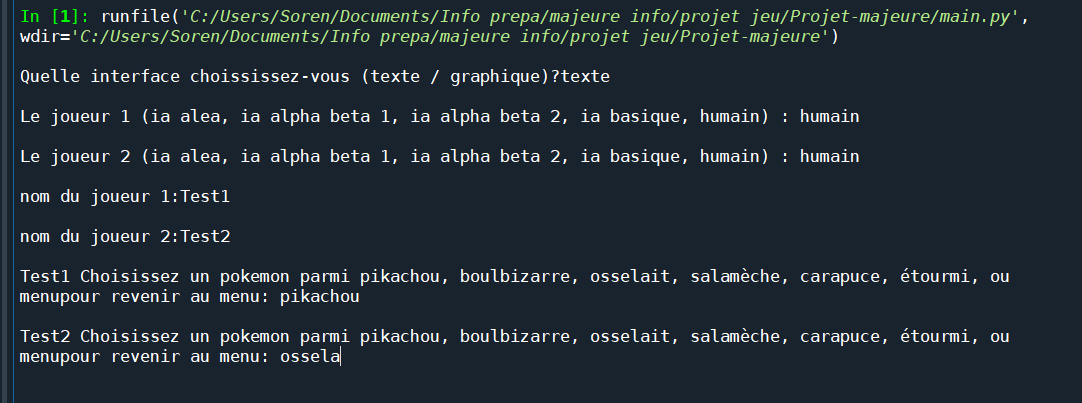
\includegraphics[width=16cm,height=6cm]{images/text1}

                Image 2: Choix lors d'un tour
                
                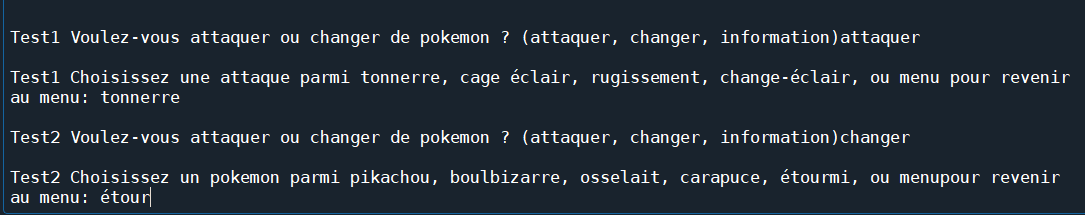
\includegraphics[width=16cm,height=6cm]{images/text2}

                Image 3 : Fin du tour
                
                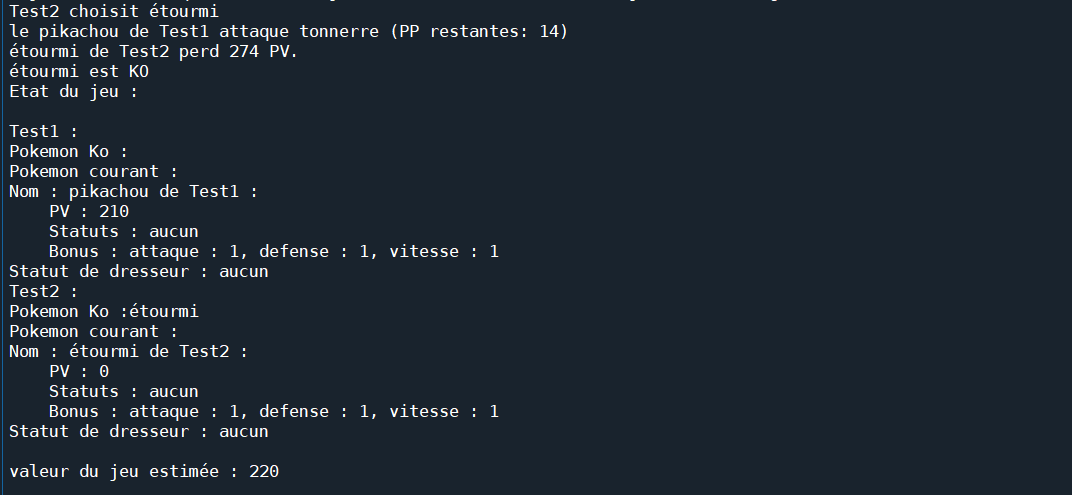
\includegraphics[width=16cm,height=6cm]{images/text3}

                Image4 : Fin de la partie
                
                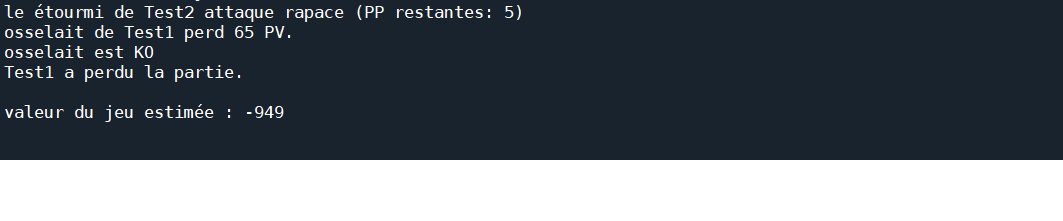
\includegraphics[width=16cm,height=6cm]{images/text4}
                

            \bigskip
    \subsection{Interface Graphique}
        L'interface graphique reprends donc la même structure que l'interface textuelle. Cependant, dans le cas de l'interface graphique, le joueur éffectue ses choix via des boutons ou des zones de texte apparaissant sur la fenêtre du jeu et non plus directement via la console. Le jeu se joue donc sur une fenêtre générée par le programme avec, sur la partie gauche, un decor ou apparaissent les pokemons actuels des deux joueurs ainsi qu'une partie sur la droite servant pour effectuer les choix/afficher les informations relatives au jeu. La nature de ces parties vous sera détaillée dans le point 6.3.2.
        Afin de pouvoir récupérer les choix des joueurs, on utilise les fonctions waitvariable et waitwindow qui nous permettent, via les fonctions liées aux boutons qui affectent ainsi une certaine valeure a la variable récupérée par le programme, de mettre celui-ci en suspent tant que le bouton n'est pas cliqué. 
        
        
        
        \subsubsection{déroulé d'un tour}
            Comme pour l'interface textuelle, il faut d'abord définir le type, le nom et le premier pokemon des deux joueurs. Pour le type et le premier pokemon, un simple clic sur le bouton voulu suffit. Pour ce qui est du nom, une zone de texte apparaît avec 'nom du joueur' en valeure par défaut. Il suffit de supprimer ce texte, de taper le pseudo voulut et d'appuyer sur la touche 'entrée' du clavier pour valider.(cf image 1, 2, 3 au point 6.3.2)

            \bigskip

            Pour chaque tour (un récapitulatif des choix respectifs des deux joueurs apparait quelques secondes si il s'agit du premier tour), comme pour l'interface textuelle, les deux joueurs choisissent entre attaquer, changer, ou avoir des informations avant de faire ce choix. Ici, ces choix se gèrent grâce à des boutons à cliquer.(cf image 4, 5, 6, 7 au point 6.3.2)

            \bigskip

             Une fois ces choix éffectués, ils s'appliquent et un récapitulatif des actions réalisées et des nouvelles informations apparaît pendant quelques secondes.(cf image 8 au point 6.3.2)

             \bigskip

             Enfin, lorsque qu'un joueur n'a plus de pokemon en état de combattre, les informations récapitulant le dernier tour apparaissent avec un message annoncant le vainqueur et la fin de la partie.(cf image 9 au point 6.3.2)

             \bigskip
            
        \subsubsection{affichages graphiques:}
            La fenêtre générée est crée via le module Tkinter. Elle est composée de 2 frames, une grande à gauche et une autre plus petite à droite. Dans notre programme, la fenêtre est définie dans le fichier fenêtre avant d'être initialisée en tant qu'attribut de la classe InterfaceGraphique. Nous tenons à préciser que nous avons essayé de reprendre au mieux l'interface de combat graphique des jeux pokemons originaux ainsi que des images issus des premiers jeux de la license pour ce qui concerne les pokemons et le decor notamment.
            \begin{itemize}
                \item La grande frame de gauche est dédiée au décor du jeu. Elle contient un grand canva qui la recouvre entièrement, dans lequel on implémente l'image servant de paysage de fond à notre jeu. Sur ce canva sont disposés, lors du choix des pokémons, 2 canvas contenant les images (sprites) des pokemons des deux joueurs. Le joueur 1 se situe en bas à droite, de dos, tandis que le joueur 2 se situe en haut à gauche, de face.Lors d'un changement de pokemon, le canva du pokemon concerné est détruit et remplacé par un nouveau contenant le nouveau pokemon.

                \item La frame de droite, elle, sert d'interface entre l'utilisateur et le jeu et d'endroit pour afficher les informations du jeu. Cette frame est en réalité un objet d'une des classes ci-dessous:
                \begin{itemize}
                    \item IHM, frame permettant de faire le choix attaquer, changer ou information.
                    \item Attaquef, frame correspondant au choix attaquer.
                    \item Changerpoke, frame correspondant au choix de changer de pokemon.
                    Information, frame correspondant au choix information.
                    \item Demandernom, frame correspondant au choix de pseudo en début de partie.
                    \item Choixjoueur, frame correspondant au choix du type de joueur en début de partie.
                    \item Etatjeu, frame affichant l'etat du jeu entre les tours.
                \end{itemize}
                A chaque changement de frame, celle-ci est détruite puis remplacée par une nouvelle instance d'une des classes ci-dessus.
            \end{itemize}
            
            \bigskip

            Pour ce qui est des boutons, ils sont crées via Tkinter et sont liés à une fonction qui permet d'affecter une certaine valeure à l'attribut 'choix' de la fenêtre qui est par la suite récupérée et traitée par l'interface. Le fonctionnement est simililaire pour le champs de texte permettant de renseigner le pseudo des joueurs en début de partie, qui est un Widget Entry de Tkinter affectant la valeure reçue lors de la pression de la touche 'entrée' à l'attribut 'choix' de la fenêtre.

            Voici quelques images pour l'interface graphique:
            Image 1: début de partie
        
            \includegraphics[width=13cm,height=7cm]{images/debut\_partie}
            
            Image 2 : choix des noms :
            
            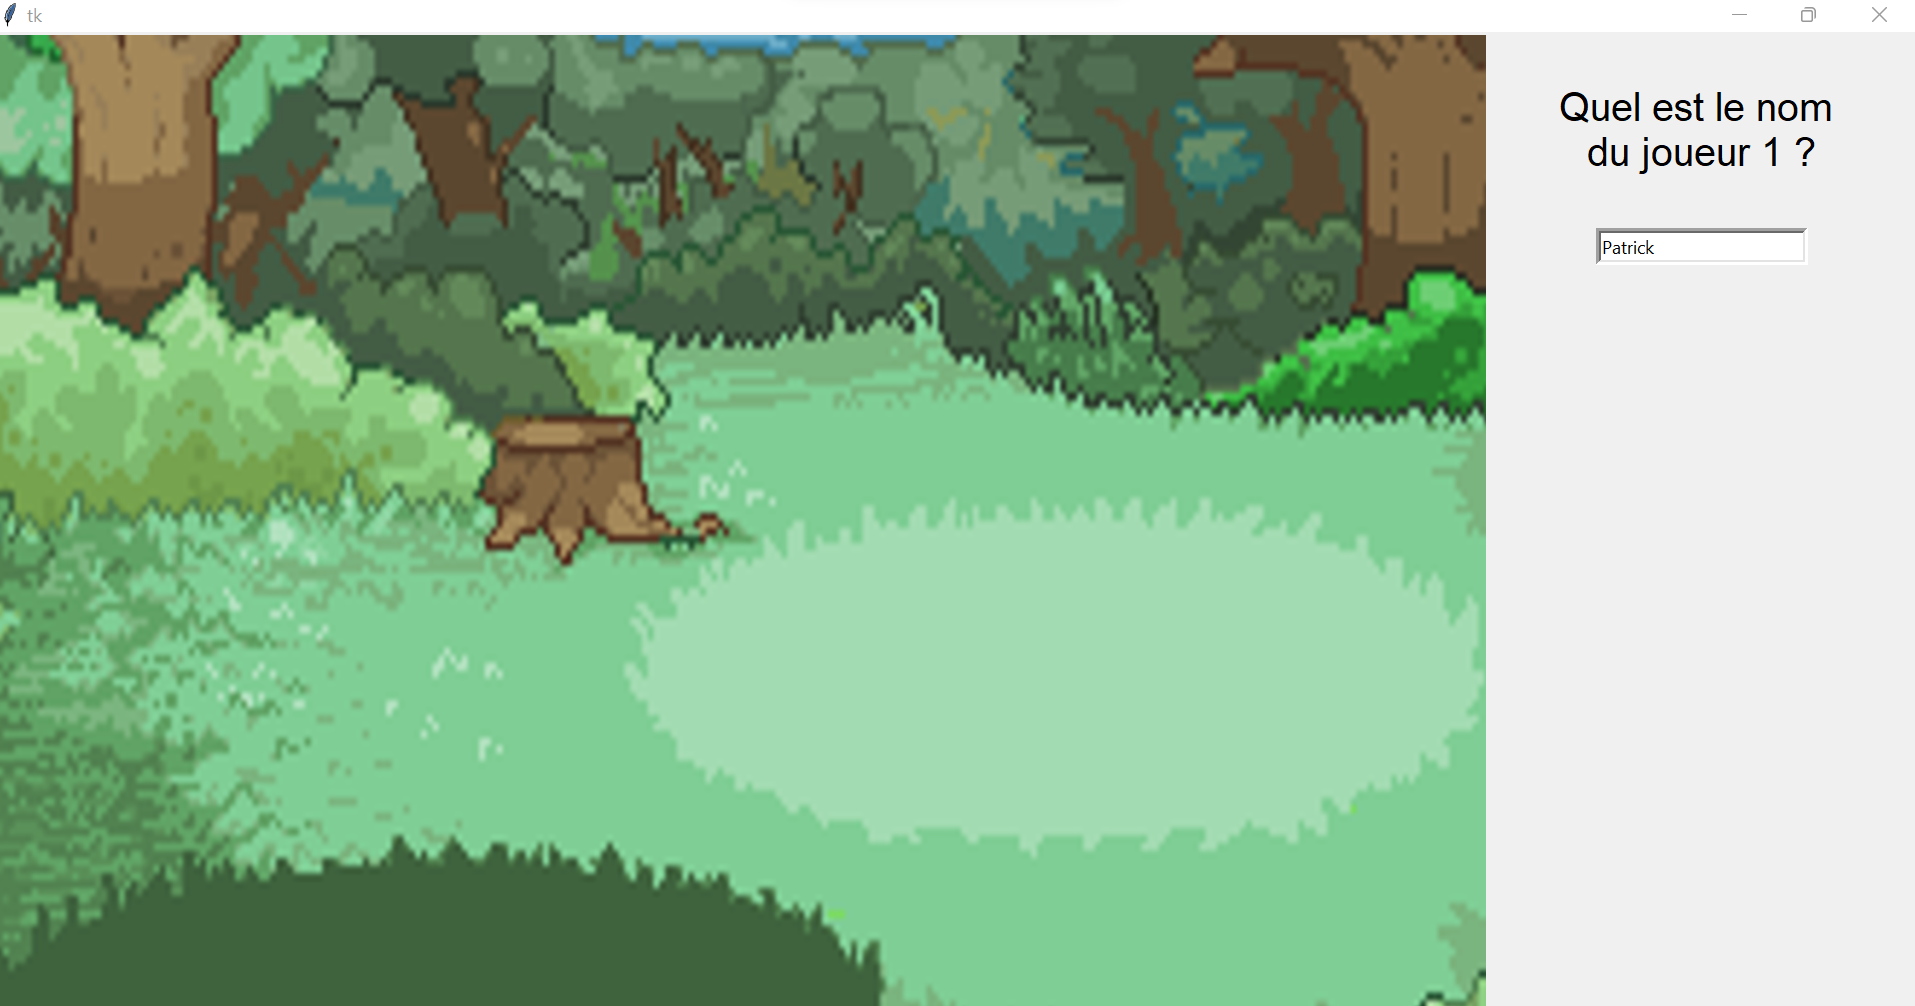
\includegraphics[width=13cm,height=7cm]{images/nom}
            
            Image 3: choix premier pokemon:
            
            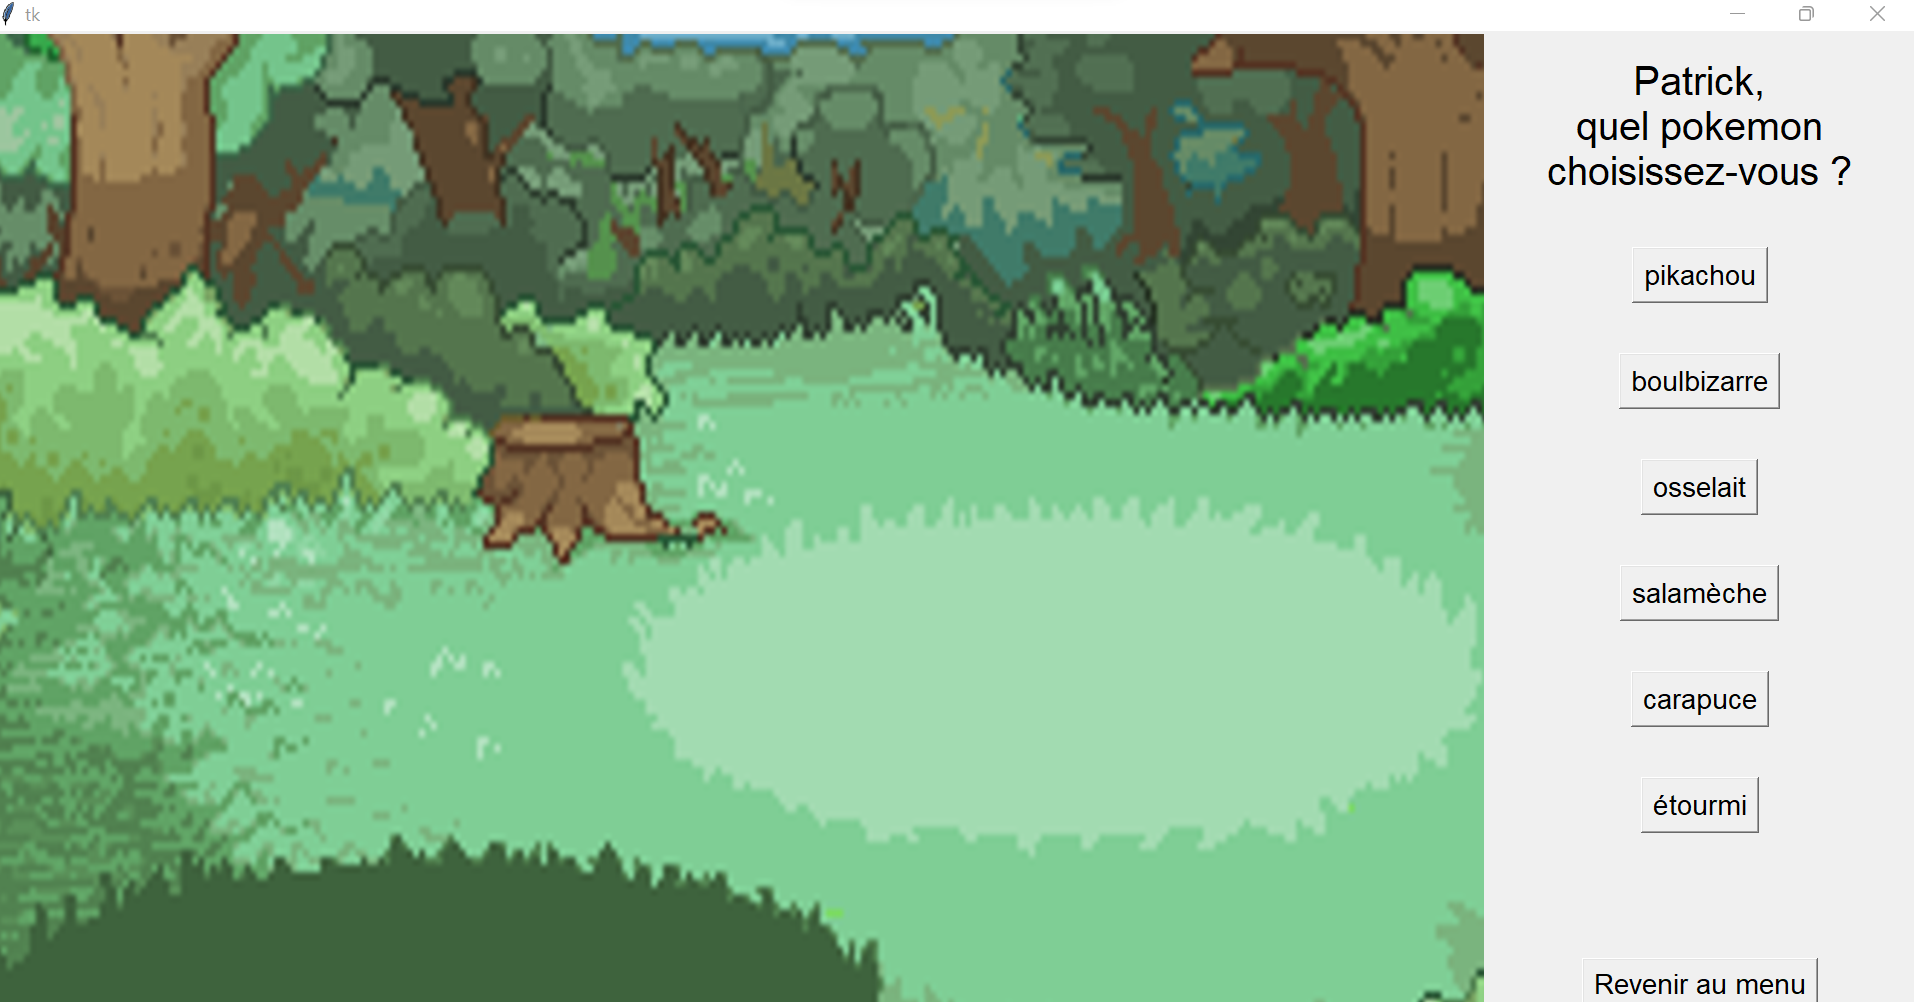
\includegraphics[width=13cm,height=7cm]{images/choix1}
            
            Image 4 : choix action :
            
            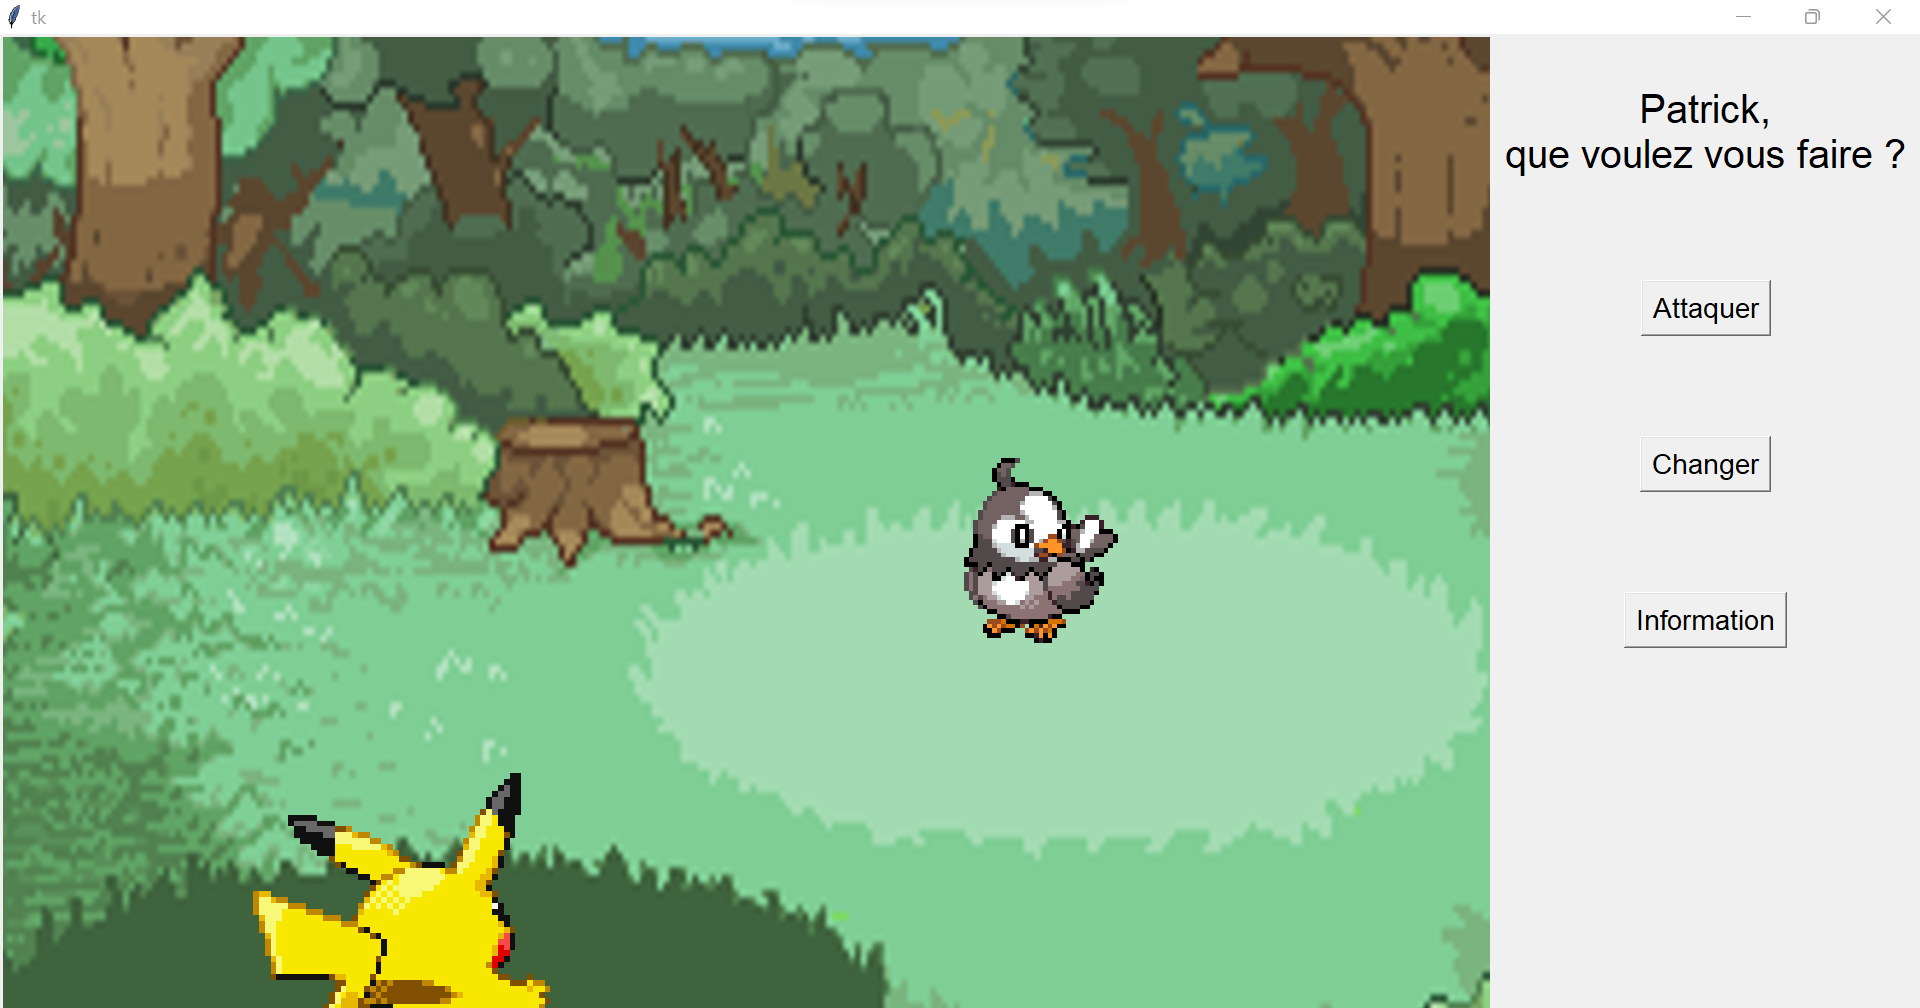
\includegraphics[width=13cm,height=7cm]{images/choix_action}
            
            Image 5 : choix des pokemons :
            
            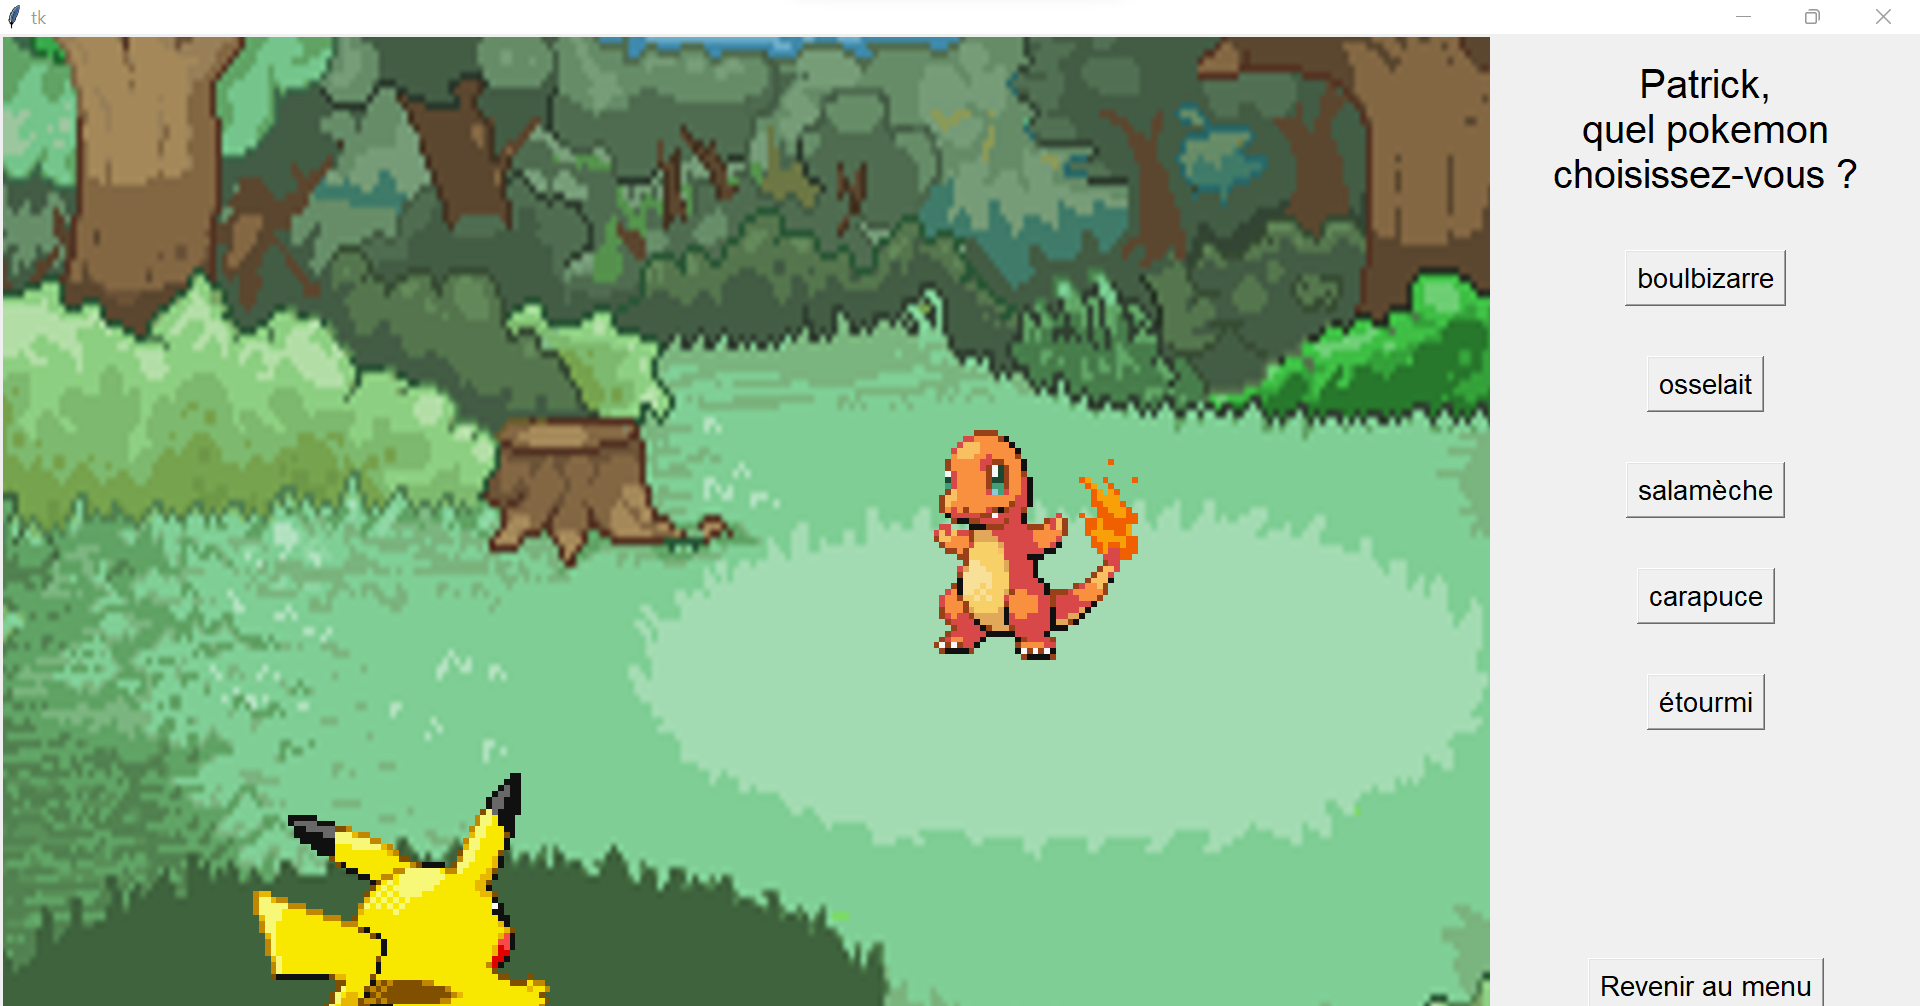
\includegraphics[width=13cm,height=7cm]{images/choix_poke}
            
            Image 6 : choix des attaques :
            
            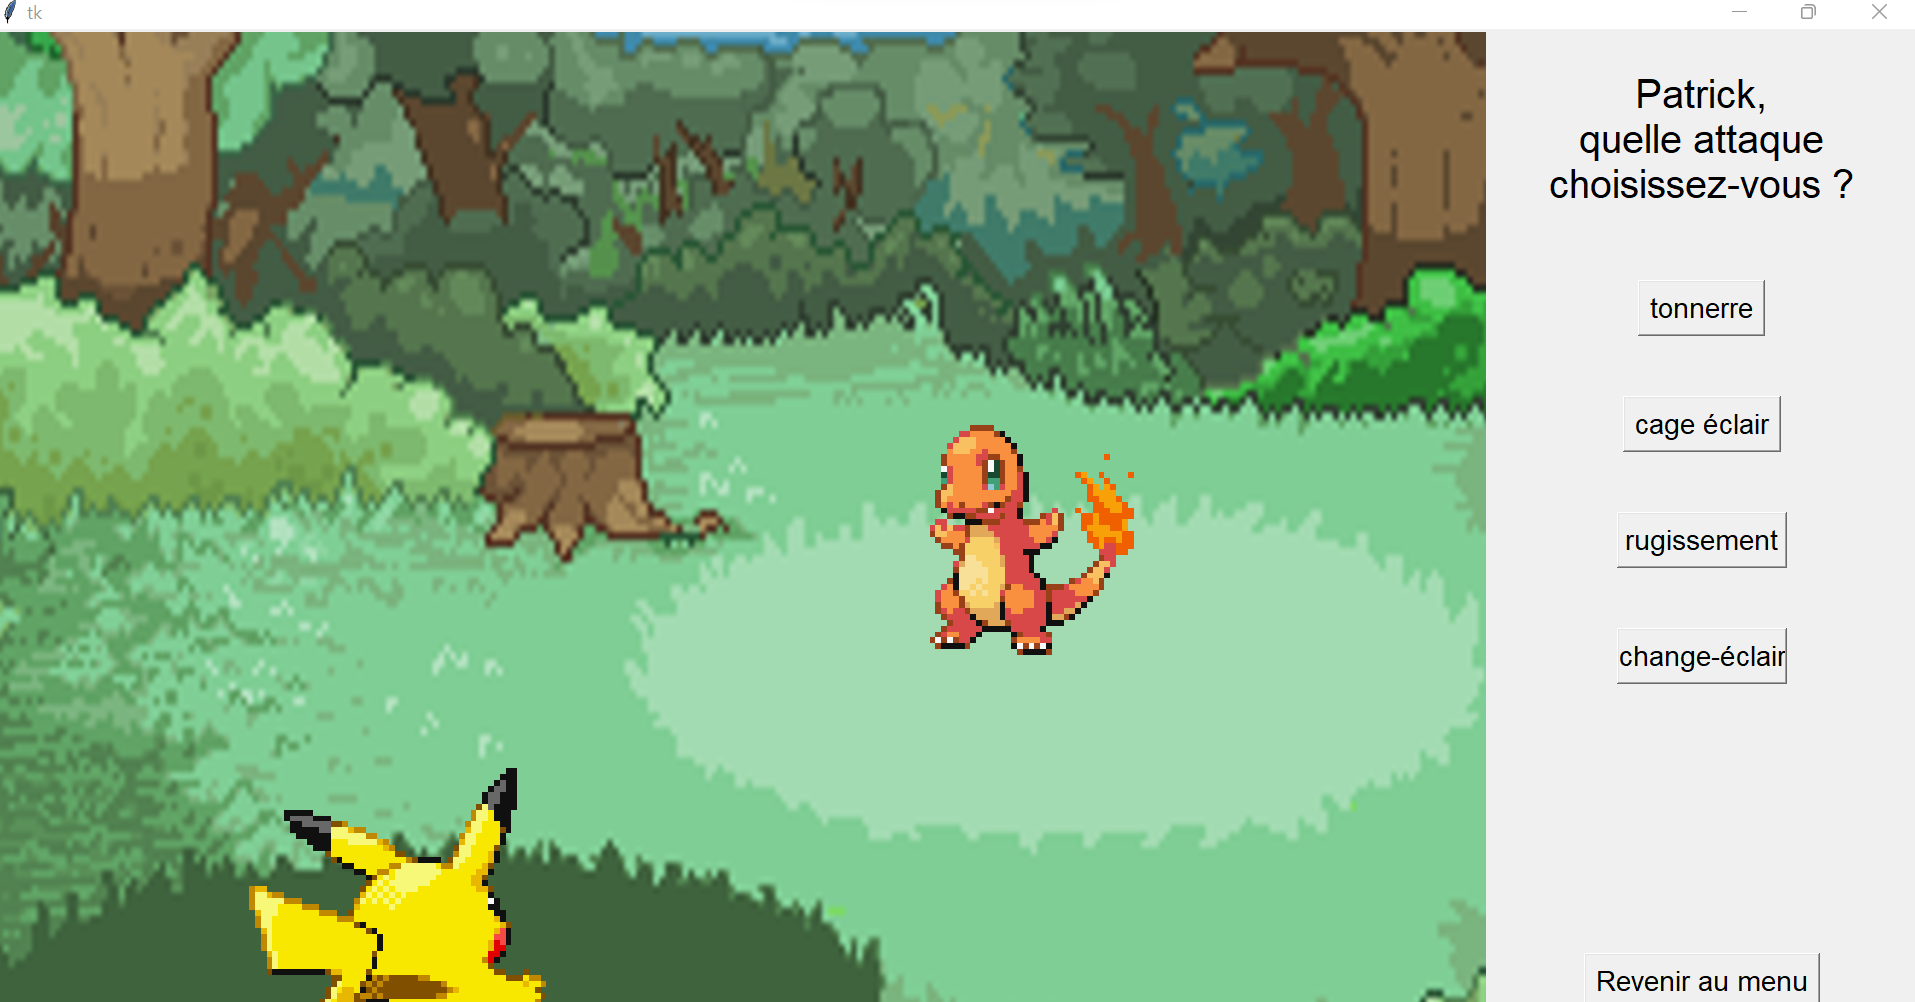
\includegraphics[width=13cm,height=7cm]{images/attaque}
            
            Images 7 : information:
            
            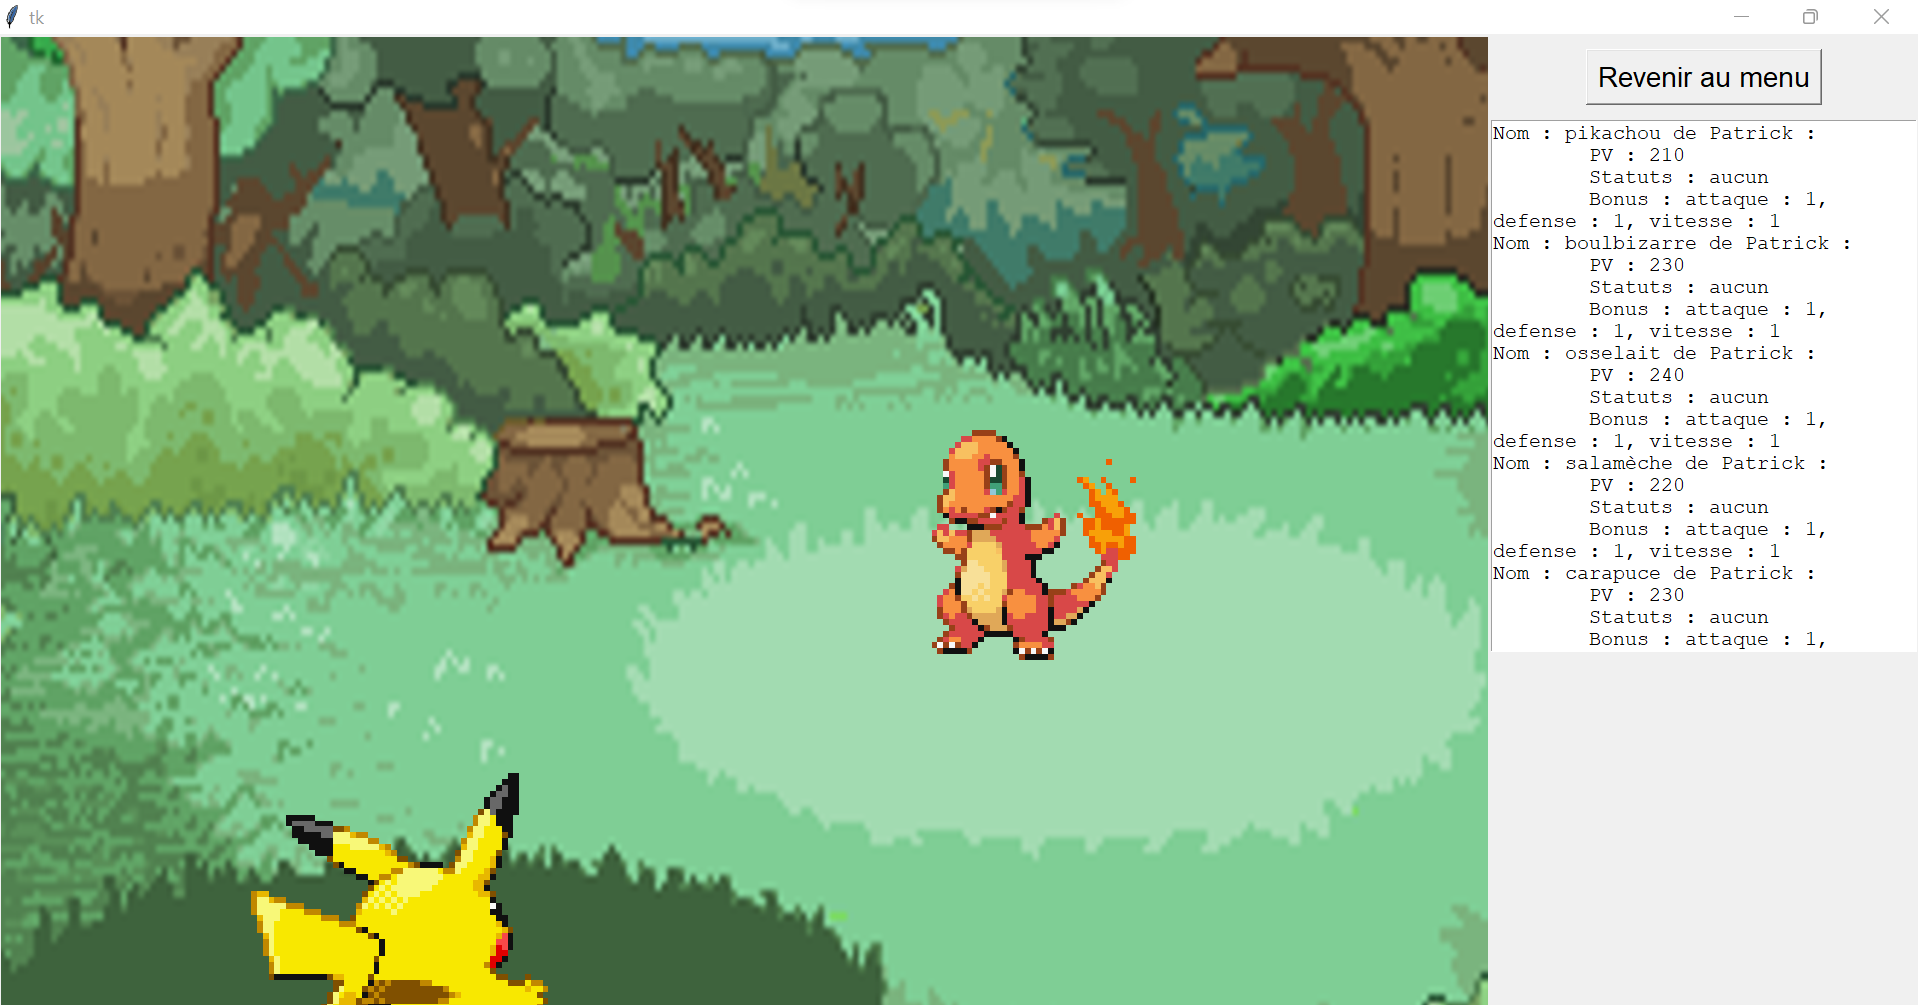
\includegraphics[width=13cm,height=7cm]{images/information}
            
            Images 8 : état du tour:
            
            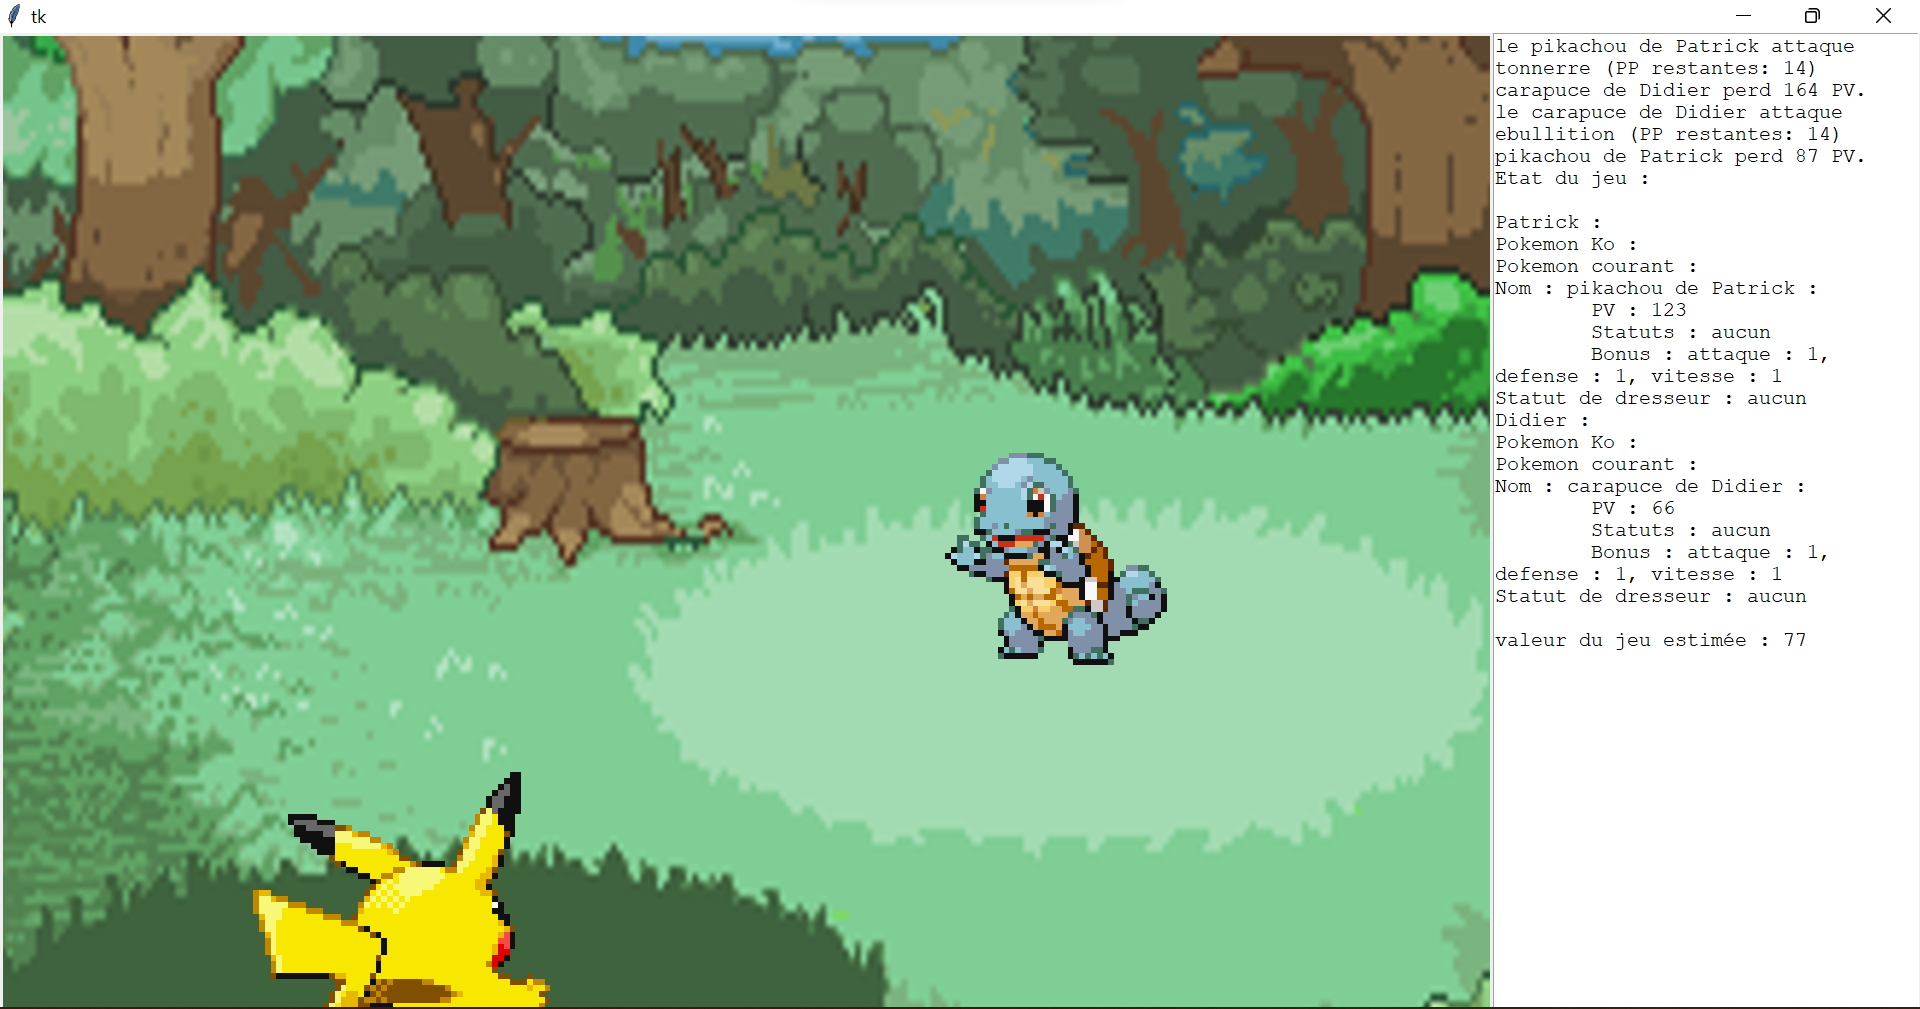
\includegraphics[width=13cm,height=7cm]{images/etat_tour}
            
            Images 9 : Fin de la partie:
            
            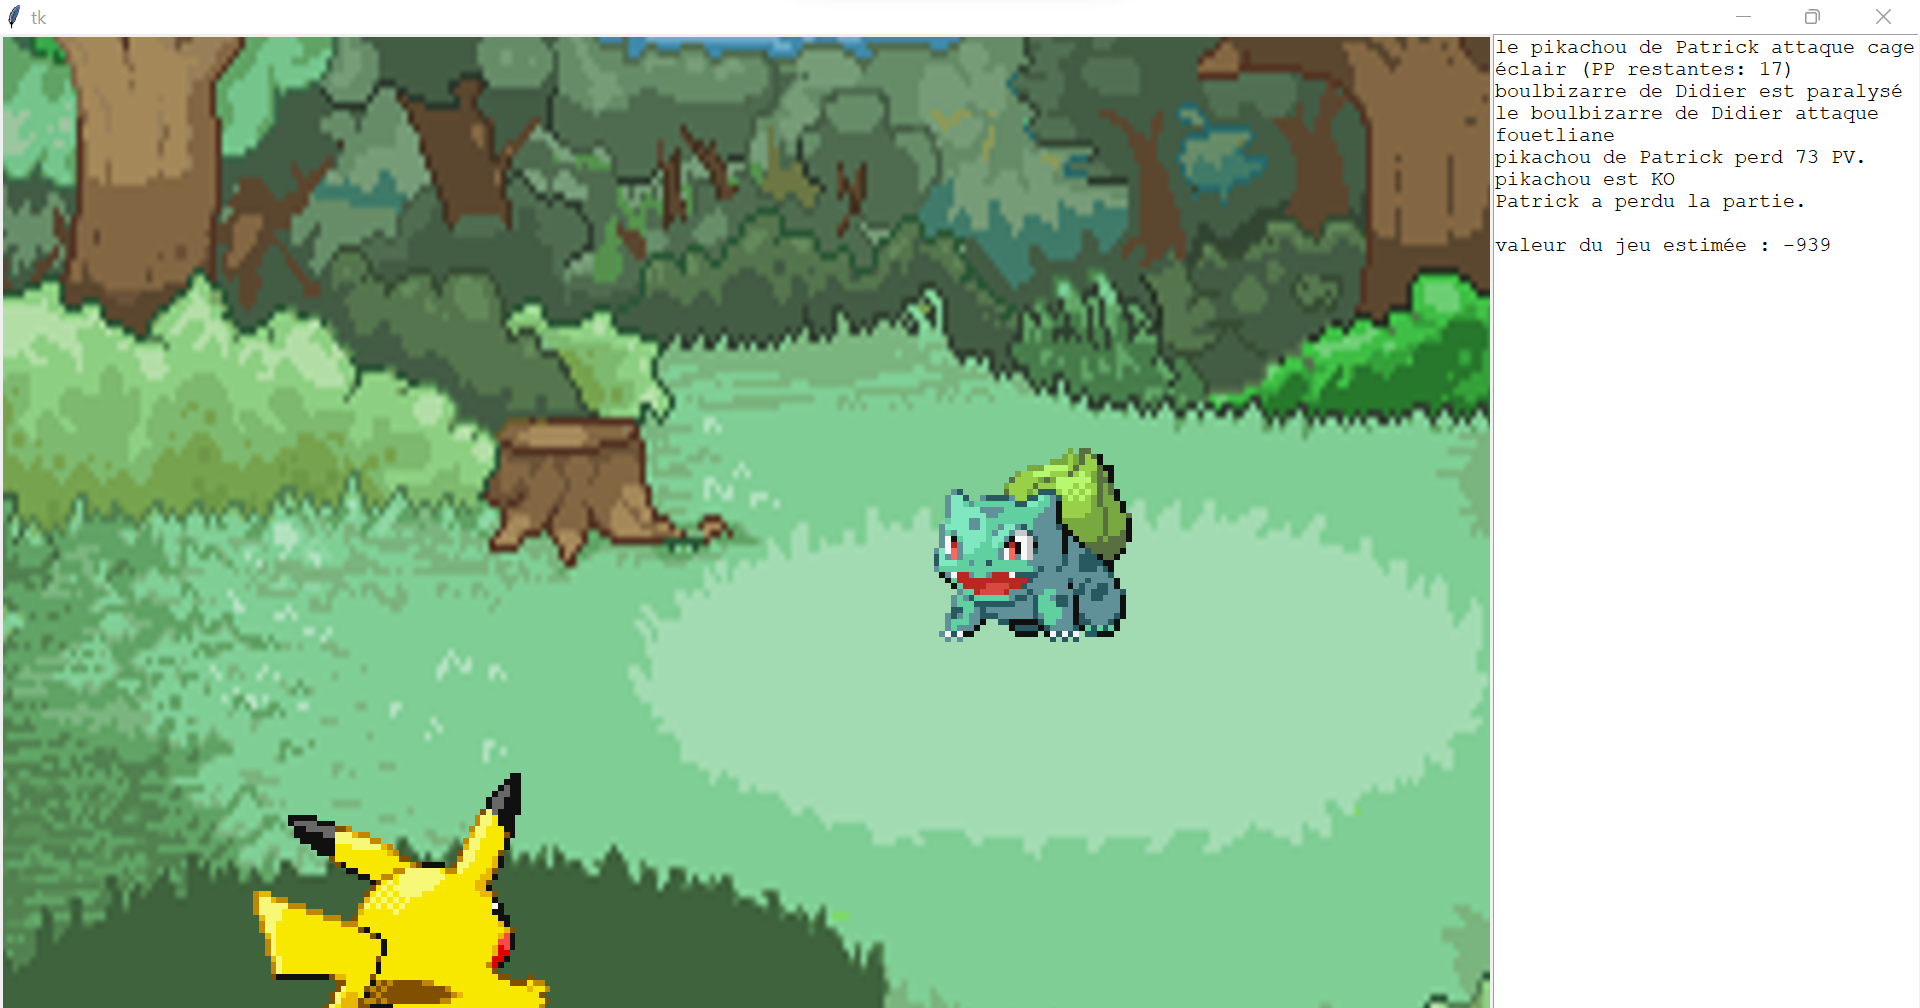
\includegraphics[width=13cm,height=7cm]{images/fin_partie}

            
        
    
        